\documentclass[tikz,border=3pt]{standalone}
\usepackage{xcolor}
\usetikzlibrary{arrows.meta,decorations.pathmorphing,positioning}
\definecolor{signalblue}{HTML}{2563EB}
\definecolor{alarmred}{HTML}{DC2626}
\definecolor{panelgray}{HTML}{E2E8F0}
\begin{document}
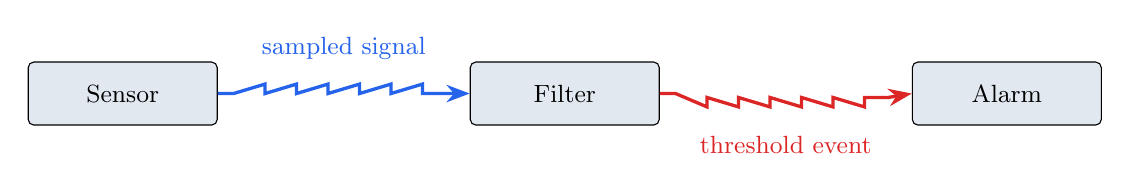
\begin{tikzpicture}[
  >=Stealth,
  process/.style={draw,rounded corners=2pt,minimum width=2.4cm,minimum height=8mm,fill=panelgray},
  every node/.style={font=\small}
]
  \node[process] (sensor) {Sensor};
  \node[process,right=3.2cm of sensor] (filter) {Filter};
  \node[process,right=3.2cm of filter] (alarm) {Alarm};
  \draw[signalblue,very thick,-Stealth,decorate,
    decoration={saw,segment length=4mm,amplitude=1.2mm,pre length=2mm,post length=3mm}]
    (sensor) -- node[above=3mm]{sampled signal} (filter);
  \draw[alarmred,very thick,-Stealth,decorate,
    decoration={saw,segment length=4mm,amplitude=1.2mm,mirror,raise=.5mm,pre length=2mm,post length=3mm}]
    (filter) -- node[below=4mm]{threshold event} (alarm);
\end{tikzpicture}
\end{document}
